\chapter{Stack}

\section{Introduction}
A \textbf{stack} is a fundamental abstract data type that operates on the Last In First Out (LIFO) principle. In other words, the last element added to the stack is the first one to be removed. Stacks are widely used in various computing applications, including expression evaluation, recursion management, and backtracking algorithms.

\section{Definition and Theoretical Background}
A stack supports the following primary operations:
\begin{itemize}
    \item \textbf{Push}: Add an element to the top of the stack.
    \item \textbf{Pop}: Remove the element from the top of the stack.
    \item \textbf{Top/Peek}: Retrieve the top element without removing it.
    \item \textbf{IsEmpty}: Check whether the stack is empty.
\end{itemize}

Formally, a stack \( S \) can be defined as a tuple \( (D, P) \), where:
\begin{itemize}
    \item \( D \) is a finite set of data elements.
    \item \( P \) is a pointer or index indicating the top element in the stack.
\end{itemize}

The operations are defined as:
\begin{itemize}
    \item \textbf{Push}: For a stack \( S = (D, P) \), pushing an element \( x \) transforms it into \( S' = (D \cup \{x\}, x) \). The new element becomes the top element.
    \item \textbf{Pop}: Removing the top element \( x \) from \( S \) results in a new stack \( S' = (D \setminus \{x\}, y) \), where \( y \) is now the top element.
    \item \textbf{Top/Peek}: This operation retrieves \( x \) (the current top element) without modifying the stack.
    \item \textbf{IsEmpty}: A boolean function that returns true if no elements are in \( D \) (i.e., \( P \) is undefined or negative).
\end{itemize}

\subsection{Additional Theoretical Considerations}
There are two common ways to implement a stack:
\begin{itemize}
    \item \textbf{Array-based Implementation}: Uses a fixed-size array to store elements. It is simple and fast but has a size limitation.
    \item \textbf{Linked List Implementation}: Uses nodes where each node points to the next element. It can grow dynamically, although it may incur extra memory overhead.
\end{itemize}

Understanding these two implementations is essential because each has its own performance characteristics and trade-offs in terms of time and space complexity.

\section{Diagrams of Stack Operations}

\subsection{Overall Stack Structure}
The following diagram shows a simple stack with three elements. The top element is at the uppermost position:
\begin{center}
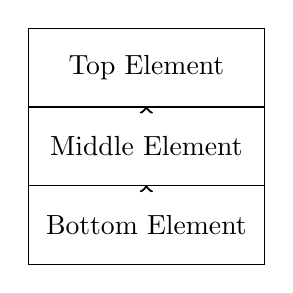
\begin{tikzpicture}[node distance=1cm]
    % Nodes representing stack elements
    \node (top) [draw, rectangle, minimum width=3cm, minimum height=1cm] {Top Element};
    \node (middle) [draw, rectangle, below of=top, minimum width=3cm, minimum height=1cm] {Middle Element};
    \node (bottom) [draw, rectangle, below of=middle, minimum width=3cm, minimum height=1cm] {Bottom Element};

    % Arrows showing order
    \draw[->, thick] (top.south) -- (middle.north);
    \draw[->, thick] (middle.south) -- (bottom.north);
\end{tikzpicture}
\end{center}

\subsection{Push Operation Diagram}
The diagram below illustrates a push operation. A new element is inserted and becomes the new top:
\begin{center}
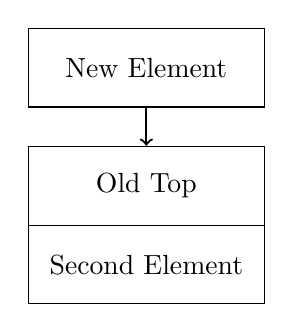
\begin{tikzpicture}[node distance=1cm]
    % Before push
    \node (oldtop) [draw, rectangle, minimum width=3cm, minimum height=1cm] {Old Top};
    \node (below) [draw, rectangle, below of=oldtop, minimum width=3cm, minimum height=1cm] {Second Element};

    % New element coming in
    \node (newelem) [draw, rectangle, minimum width=3cm, minimum height=1cm, above of=oldtop, node distance=1.5cm] {New Element};

    % Arrows to indicate push
    \draw[->, thick] (newelem.south) -- (oldtop.north);
\end{tikzpicture}
\end{center}

\subsection{Pop Operation Diagram}
The following diagram shows the pop operation, where the top element is removed:
\begin{center}
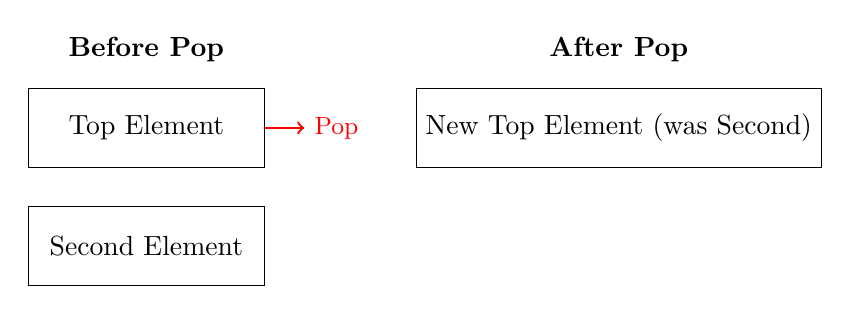
\begin{tikzpicture}[node distance=1cm]

% --- Stack BEFORE pop ---
\node at (0, 2.5) {\textbf{Before Pop}};
\node (before_top) [draw, rectangle, minimum width=3cm, minimum height=1cm] at (0,1.5) {Top Element};
\node (before_second) [draw, rectangle, minimum width=3cm, minimum height=1cm] at (0,0) {Second Element};
\draw[->, thick, red] (before_top.east) -- ++(0.5,0) node[right]{\small Pop};

% --- Stack AFTER pop ---
\node at (6, 2.5) {\textbf{After Pop}};
\node (after_top) [draw, rectangle, minimum width=3cm, minimum height=1cm] at (6,1.5) {New Top Element (was Second)};

\end{tikzpicture}
\end{center}


\section{C++ Implementation of a Stack}
Below is an extended implementation of a stack using an array in C++ with additional inline comments for clarity.

\begin{lstlisting}[caption={C++ implementation of a Stack using an array}]
#include <bits/stdc++.h>
#define MAX 100

class Stack {
private:
    int arr[MAX]; // Array to store stack elements
    int top;      // Index of the top element
public:
    // Constructor initializes top to -1 indicating an empty stack
    Stack() : top(-1) {}

    // Check if the stack is empty
    bool isEmpty() {
        return (top < 0);
    }
    // Push an element onto the stack
    bool push(int x) {
        if(top >= (MAX - 1)) {
            cout << "Stack Overflow" << "\n";
            return false;
        } else {
            arr[++top] = x;
            return true;
        }
    }
    // Pop an element from the stack
    int pop() {
        if(isEmpty()){
            cout << "Stack Underflow" << "\n";
            return -1;
        } else {
            int x = arr[top--];
            return x;
        }
    }
    // Peek at the top element without removing it
    int peek() {
        if(isEmpty()){
            cout << "Stack is Empty" << "\n";
            return -1;
        } else {
            return arr[top];
        }
    }
};
int main() {
    Stack s;
    // Example operations on the stack
    s.push(10);   // Stack: [10]
    s.push(20);   // Stack: [10, 20]
    s.push(30);   // Stack: [10, 20, 30]
    cout << "Top element is " << s.peek() << "\n"; // Should print 30
    cout << "Popped element is " << s.pop() << "\n"; // Removes 30
    cout << "New top element is " << s.peek() << "\n"; // Should print 20

    return 0;
}
\end{lstlisting}

\section{Example Scenario in Detail}
Consider the following sequence of operations on an initially empty stack:
\begin{enumerate}
    \item \textbf{Push} 5 onto the stack. \\
          \textbf{Stack state}: [5] (5 becomes the top element)
    \item \textbf{Push} 10 onto the stack. \\
          \textbf{Stack state}: [5, 10] (10 is now at the top)
    \item \textbf{Push} 15 onto the stack. \\
          \textbf{Stack state}: [5, 10, 15] (15 becomes the new top)
    \item \textbf{Pop} the top element. \\
          \textbf{Stack state}: [5, 10] (15 is removed; 10 becomes the top)
\end{enumerate}

The above scenario is illustrated in the diagrams provided earlier. When a new element is pushed, it becomes the new top, and when an element is popped, the previous element becomes the top.

\section{Infix, Postfix, and Prefix Conversion}

Expressions can be written in three common forms:
\begin{itemize}
    \item \textbf{Infix:} The operator is written between the operands (e.g., \texttt{A + B}).
    \item \textbf{Postfix (Reverse Polish Notation):} The operator follows the operands (e.g., \texttt{A B +}).
    \item \textbf{Prefix (Polish Notation):} The operator precedes the operands (e.g., \texttt{+ A B}).
\end{itemize}

\subsection{Theory and Conversion Algorithms}
To convert an infix expression to postfix, follow these steps:
\begin{enumerate}
    \item Scan the infix expression from left to right.
    \item Use a stack to store operators and an output string for the result.
    \item When an operand (letter or number) is encountered, append it to the output.
    \item When an operator is encountered, pop from the stack to the output until either the stack is empty or the operator at the top of the stack has lower precedence than the current operator. Then, push the current operator onto the stack.
    \item When a left parenthesis \texttt{(} is encountered, push it onto the stack.
    \item When a right parenthesis \texttt{)} is encountered, pop from the stack to the output until a left parenthesis is encountered; then discard the pair of parentheses.
    \item After processing the entire expression, pop any remaining operators from the stack to the output.
\end{enumerate}

For \textbf{infix to prefix conversion}, a common method is:
\begin{itemize}
    \item Reverse the infix expression.
    \item Swap every \texttt{(} with \texttt{)} and vice-versa.
    \item Convert the modified expression to postfix.
    \item Reverse the resulting postfix expression to obtain the prefix expression.
\end{itemize}

\subsection{Extended C++ Implementation}

Below is an extended C++ code that implements both infix-to-postfix and infix-to-prefix conversion. Notice the use of helper functions to reverse strings and swap parentheses.

\begin{lstlisting}[language=C++, caption={Extended C++ Code for Infix, Postfix, and Prefix Conversion}]
#include <bits/stdc++.h>

using namespace std;

// Function to return precedence of operators
int precedence(char op) {
    if(op == '+' || op == '-') return 1;
    if(op == '*' || op == '/') return 2;
    return 0;
}
// Infix to Postfix conversion
string infixToPostfix(const string &infix) {
    string postfix;
    stack<char> s;
    for (char c : infix) {
        // If the character is an operand, append it to output
        if(isalnum(c))
            postfix += c;
        // If '(' encountered, push to stack
        else if(c == '(')
            s.push(c);
        // If ')' encountered, pop until '('
        else if(c == ')') {
            while(!s.empty() && s.top() != '(') {
                postfix += s.top();
                s.pop();
            }
            if(!s.empty())
                s.pop(); // pop '('
        }
        // If operator encountered
        else {
            while(!s.empty() && precedence(c) <= precedence(s.top())) {
                postfix += s.top();
                s.pop();
            }
            s.push(c);
        }
    }
    // Pop remaining operators
    while(!s.empty()) {
        postfix += s.top();
        s.pop();
    }
    return postfix;
}
// Utility function to reverse a string
string reverseString(string s) {
    reverse(s.begin(), s.end());
    return s;
}
// Swap parentheses in a string
string swapParentheses(string s) {
    for (char &c : s) {
        if(c == '(') c = ')';
        else if(c == ')') c = '(';
    }
    return s;
}

// Infix to Prefix conversion using reverse-process method
string infixToPrefix(string infix) {
    // Reverse the infix expression and swap parentheses
    string rev = reverseString(infix);
    rev = swapParentheses(rev);
    // Convert reversed expression to postfix
    string revPostfix = infixToPostfix(rev);
    // Reverse the postfix expression to get prefix
    string prefix = reverseString(revPostfix);
    return prefix;
}

int main() {
    // Example 1
    string infix1 = "((A+B)*C)-(D/E)";
    cout << "Infix 1: " << infix1 << endl;
    cout << "Postfix 1: " << infixToPostfix(infix1) << endl;
    cout << "Prefix 1: " << infixToPrefix(infix1) << endl << endl;
    
    // Example 2
    string infix2 = "A*(B+C)/D";
    cout << "Infix 2: " << infix2 << endl;
    cout << "Postfix 2: " << infixToPostfix(infix2) << endl;
    cout << "Prefix 2: " << infixToPrefix(infix2) << endl;
    
    return 0;
}
\end{lstlisting}

\subsection{Expression Tree Diagrams}

The following diagrams represent the expression trees for the given expressions. These trees help visualize how the expressions are structured and how different traversals yield the infix, postfix, and prefix notations.

\subsubsection*{Example 1: \( ((A+B)*C)-(D/E) \)}

\textbf{Expression Tree:}

\begin{center}
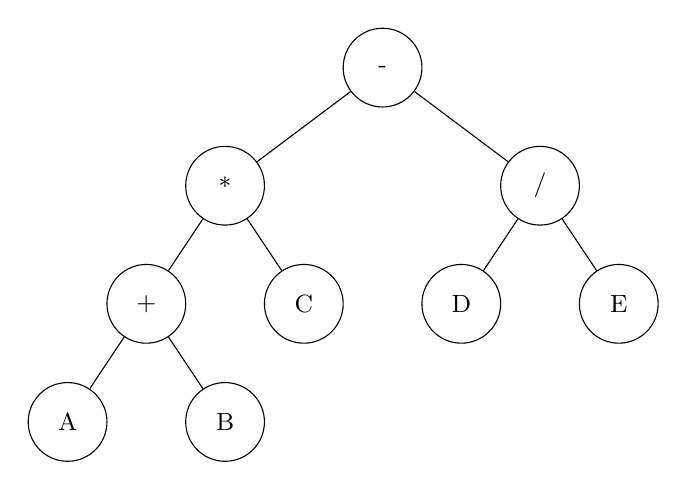
\begin{tikzpicture}[level distance=1.5cm,
  level 1/.style={sibling distance=4cm},
  level 2/.style={sibling distance=2cm},
  every node/.style={draw, circle, minimum size=1cm, font=\small}]
  \node { - }
    child { node { * }
      child { node { + }
        child { node { A } }
        child { node { B } }
      }
      child { node { C } }
    }
    child { node { / }
      child { node { D } }
      child { node { E } }
    };
\end{tikzpicture}
\end{center}

\textbf{Traversals:}
\begin{itemize}
    \item \textbf{Inorder (Infix):} \( ((A+B)*C)-(D/E) \)
    \item \textbf{Postorder (Postfix):} \( A\,B\,+\,C\,*\,D\,E\,/\,- \)
    \item \textbf{Preorder (Prefix):} \( -\,*\,+\,A\,B\,C\,/\,D\,E \)
\end{itemize}

\subsubsection*{Example 2: \( A*(B+C)/D \)}

\textbf{Expression Tree:}

\begin{center}
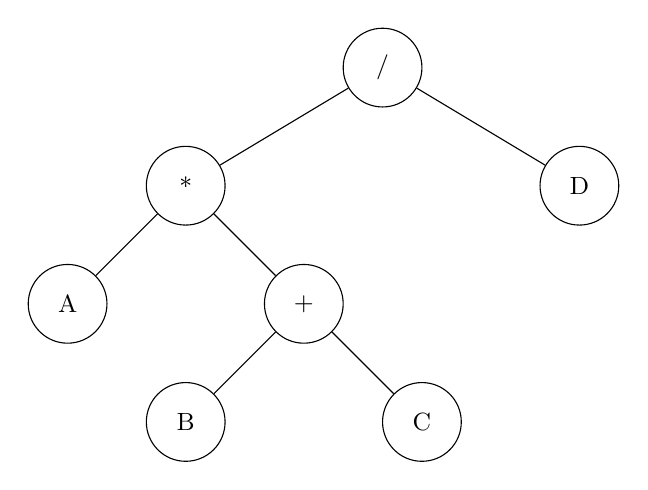
\begin{tikzpicture}[level distance=1.5cm,
  level 1/.style={sibling distance=5cm},
  level 2/.style={sibling distance=3cm},
  every node/.style={draw, circle, minimum size=1cm, font=\small}]
  \node { / }
    child { node { * }
      child { node { A } }
      child { node { + }
        child { node { B } }
        child { node { C } }
      }
    }
    child { node { D } };
\end{tikzpicture}
\end{center}

\textbf{Traversals:}
\begin{itemize}
    \item \textbf{Inorder (Infix):} \( A*(B+C)/D \)
    \item \textbf{Postorder (Postfix):} \( A\,B\,C\,+\,*\,D\,/ \)
    \item \textbf{Preorder (Prefix):} \( /\,*\,A\,+\,B\,C\,D \)
\end{itemize}

\medskip
This section has provided detailed theory, extended C++ implementations, additional examples, and visual diagrams. With these tools, you should be able to understand and implement conversions between infix, postfix, and prefix notations effectively.


\section{C++ Implementation of a Stack using Linked List}

Unlike the array-based stack, a linked list implementation does not have a fixed size. It can grow and shrink dynamically as needed. Each node in the linked list stores a value and a pointer to the next node.

\begin{lstlisting}[caption={C++ implementation of a Stack using a Linked List}]
#include <bits/stdc++.h>
using namespace std;

class Node {
public:
    int data;
    Node* next;
};

class StackLL {
private:
    Node* top;

public:
    // Constructor
    StackLL() {
        top = nullptr;
    }
    // Push operation
    void push(int x) {
        Node* temp = new Node();
        if (!temp) {
            cout << "Heap Overflow\n";
            return;
        }
        temp->data = x;
        temp->next = top;
        top = temp;
    }
    // Check if the stack is empty
    bool isEmpty() {
        return top == nullptr;
    }
    // Pop operation
    void pop() {
        if (isEmpty()) {
            cout << "Stack Underflow\n";
            return;
        }
        Node* temp = top;
        top = top->next;
        delete temp;
    }

    // Peek operation
    int peek() {
        if (!isEmpty())
            return top->data;
        else {
            cout << "Stack is Empty\n";
            return -1;
        }
    }
    // Display contents of stack
    void display() {
        if (isEmpty()) {
            cout << "Stack is empty\n";
            return;
        }
        Node* temp = top;
        while (temp != nullptr) {
            cout << temp->data << " -> ";
            temp = temp->next;
        }
        cout << "NULL\n";
    }
};
int main() {
    StackLL s;
    s.push(5);
    s.push(10);
    s.push(15);
    cout << "Top element is: " << s.peek() << "\n";
    s.pop();
    s.display();

    return 0;
}
\end{lstlisting}

This linked list-based stack grows dynamically, avoiding stack overflow unless system memory is exhausted. The `push`, `pop`, and `peek` operations each run in \( O(1) \) time, offering efficient performance and flexibility.


\section{Conclusion}
Stacks are a fundamental data structure that implements the Last In First Out (LIFO) principle. This chapter has detailed the stack's theoretical basis, explained each operation in depth, and presented multiple diagrams to visually represent the stack and its operations. Additionally, a practical C++ implementation is provided to illustrate how stacks can be implemented and used in real-world applications, such as managing function calls and evaluating expressions.